% ============================================================
%  Proyecto de Criptografía — Entrega 2 (Implementación y demo)
%  Administrador de Contraseñas Seguro (zero-knowledge)
%  Compilar con: pdflatex entrega2.tex  (2 veces)
% ============================================================
\documentclass[aspectratio=169,10pt]{beamer}

\usepackage[T1]{fontenc}
\usepackage[utf8]{inputenc}
\IfFileExists{lmodern.sty}{\usepackage{lmodern}}{}
% Carga babel-spanish solo si está disponible (Overleaf sí lo tiene)
\IfFileExists{spanish.ldf}{\usepackage[spanish,es-noshorthands]{babel}}{}
\usepackage{amsmath}
\usepackage{amssymb}
\usepackage{booktabs}
\usepackage{array}
\usepackage{listings}
\usepackage{tikz}
\usetikzlibrary{positioning,arrows.meta,fit,backgrounds,calc,shapes.geometric}

\usetheme{Madrid}
\usecolortheme{seahorse}
\setbeamertemplate{navigation symbols}{}
\setbeamertemplate{caption}[numbered]
\setbeamerfont{frametitle}{size=\large}
\setbeamercolor{structure}{fg=blue!55!black}
\setbeamertemplate{itemize items}[circle]

\definecolor{cliente}{HTML}{1B5E20}
\definecolor{servidor}{HTML}{B71C1C}
\definecolor{cripto}{HTML}{0D47A1}
\definecolor{gris}{HTML}{F2F2F2}

\newcommand{\key}[1]{\textcolor{cripto}{\texttt{#1}}}
\newcommand{\hecho}{\textcolor{cliente}{$\checkmark$}}
\newcommand{\falta}{\textcolor{servidor}{$\times$}}
\newcommand{\code}[1]{\texttt{\footnotesize #1}}

\lstset{
  basicstyle=\ttfamily\scriptsize,
  keywordstyle=\color{cripto}\bfseries,
  commentstyle=\color{gray}\itshape,
  stringstyle=\color{cliente},
  backgroundcolor=\color{gris},
  frame=single, rulecolor=\color{gray!40},
  columns=fullflexible, keepspaces=true,
  showstringspaces=false, aboveskip=2pt, belowskip=2pt,
  language=Python,
}

% --------- estilos TikZ comunes ---------
\tikzset{
  comp/.style   = {draw, rounded corners=2pt, fill=white, minimum width=34mm,
                   minimum height=8mm, align=center, font=\scriptsize},
  zone/.style   = {draw, dashed, rounded corners=5pt, inner sep=4mm, thick},
  dato/.style   = {draw, rounded corners=2pt, fill=gris, align=center, font=\scriptsize,
                   minimum height=7mm, minimum width=22mm},
  op/.style     = {draw, fill=cripto!12, rounded corners=2pt, align=center,
                   font=\scriptsize\bfseries, minimum height=7mm, minimum width=24mm},
  llave/.style  = {draw, fill=cripto!30, rounded corners=2pt, align=center,
                   font=\scriptsize\bfseries, minimum height=7mm, minimum width=20mm},
  flecha/.style = {-{Stealth[length=2mm]}, thick},
}

% ============================================================
\title[Gestor de contraseñas E2E]{Administrador de Contraseñas Seguro}
\subtitle{Entrega 2 — Implementación y demo}
\author[Pacheco · Berru]{Franco Pacheco \and Andy Rai Berru Tenorio}
\institute[UTEC]{Criptografía \\ Universidad de Ingeniería y Tecnología (UTEC)}
\date[Semana 16]{Presentación final — Semana 16}

\begin{document}

% ---------------------------------------------------------- portada
\begin{frame}[plain]
  \titlepage
\end{frame}

% ---------------------------------------------------------- agenda
\begin{frame}{Agenda}
  \small
  \begin{columns}[T]
    \begin{column}{0.5\textwidth}
      \begin{enumerate}
        \item Del diseño a la implementación
        \item Arquitectura implementada
        \item Primitivos: del diseño al código
        \item Derivación de llaves y cifrado de la bóveda
        \item Nonces, AAD y \emph{padding}
        \item Passkeys Ed25519
        \item Anti-\emph{rollback}
      \end{enumerate}
    \end{column}
    \begin{column}{0.5\textwidth}
      \begin{enumerate}
        \setcounter{enumi}{7}
        \item Cambio de contraseña maestra
        \item Seguridad en tránsito y \emph{certificate pinning}
        \item Seguridad en reposo y en el dispositivo
        \item Verificación: pruebas y análisis estático
        \item Demo
        \item Amenazas, desviaciones y limitaciones
        \item Reparto del trabajo y conclusiones
      \end{enumerate}
    \end{column}
  \end{columns}
\end{frame}

% ---------------------------------------------------------- promesa vs implementado
\begin{frame}{Del diseño a la implementación: ¿cumplimos lo prometido?}
  \centering\scriptsize
  \renewcommand{\arraystretch}{0.95}
  \begin{tabular}{@{}p{0.40\textwidth} c p{0.44\textwidth}@{}}
    \toprule
    \textbf{Prometido en la Entrega 1} & & \textbf{Implementación} \\
    \midrule
    Argon2id + HKDF + Secret Key de 256 bits & \hecho & \code{client/crypto/kdf.py}, \code{keys.py} \\
    Bóveda AEAD (XChaCha20-Poly1305) y \emph{key wrapping} de \key{VK} & \hecho & \code{aead.py}, \code{vault/blob.py} \\
    Crear, editar, duplicar, eliminar, buscar, etiquetas & \hecho & \code{vault/models.py} + UI \\
    Generador con CSPRNG y medidor de entropía & \hecho & \code{crypto/generator.py} (\code{secrets}) \\
    Servidor: registro, login, blob versionado & \hecho & FastAPI, 11 endpoints \\
    TLS 1.3 sin \emph{downgrade} & \hecho & contexto TLS con mínimo 1.3 (cliente y servidor) \\
    Passkeys Ed25519 con \emph{challenge-response} & \hecho & \code{crypto/passkeys.py}, \code{server/app/passkeys.py} \\
    Anti-\emph{rollback} (versión en el AAD) & \hecho & AAD + marca de agua local \\
    Cambio de contraseña sin re-cifrar la bóveda & \hecho & sólo se re-envuelve \key{VK} \\
    Bloqueo automático y portapapeles temporizado & \hecho & \code{ui/idle.py}, \code{ui/clipboard.py} \\
    \emph{Certificate pinning} & \hecho & pin SPKI SHA-256 (\code{net/pinning.py}) \\
    \emph{Padding} del blob, exportación cifrada & \hecho & bloques de 4\,KiB; archivo \code{.pmx} \\
    \texttt{bandit} + \texttt{semgrep} + \texttt{pip-audit} en CI & \hecho & GitHub Actions \\
    Docker Compose + PostgreSQL & \falta & SQLite por defecto (PostgreSQL vía URL) \\
    \bottomrule
  \end{tabular}

  \vspace{2mm}
  {\footnotesize \textbf{144 pruebas automáticas} · $\approx$4\,700 líneas de código · \textbf{0} hallazgos
  de \texttt{bandit} · \textbf{0} vulnerabilidades conocidas (\texttt{pip-audit})}
\end{frame}

% ---------------------------------------------------------- arquitectura
\begin{frame}{Arquitectura implementada}
  \centering
  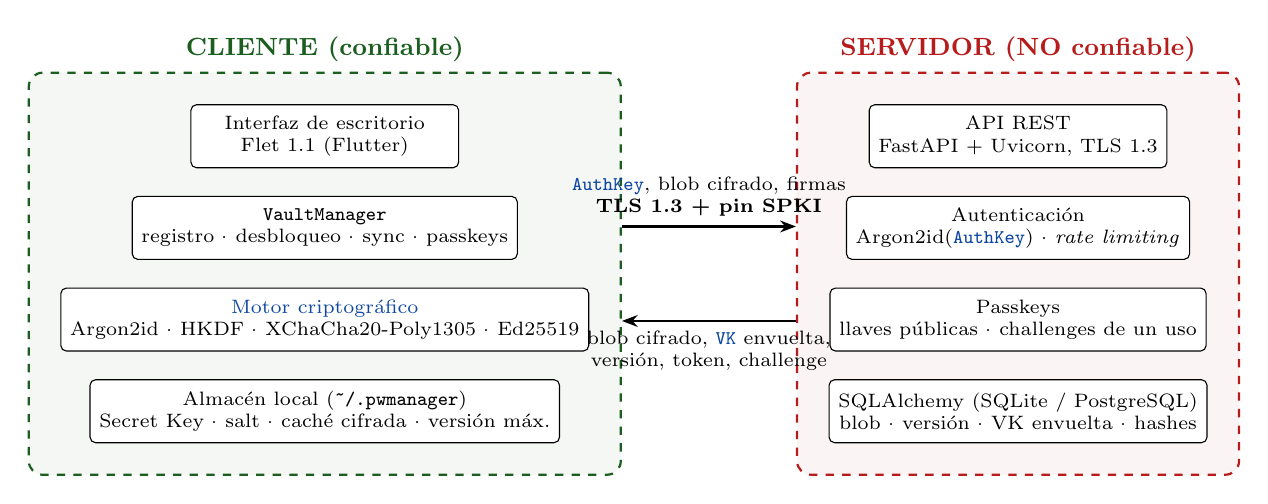
\begin{tikzpicture}[node distance=3.5mm]
    % ---- cliente
    \node[comp] (ui) {Interfaz de escritorio\\ \scriptsize Flet 1.1 (Flutter)};
    \node[comp, below=of ui] (logic) {\texttt{VaultManager}\\ \scriptsize registro · desbloqueo · sync · passkeys};
    \node[comp, below=of logic] (crypto) {\textcolor{cripto}{Motor criptográfico}\\ \scriptsize Argon2id · HKDF · XChaCha20-Poly1305 · Ed25519};
    \node[comp, below=of crypto] (local) {Almacén local (\texttt{\textasciitilde/.pwmanager})\\ \scriptsize Secret Key · salt · caché cifrada · versión máx.};
    \begin{scope}[on background layer]
      \node[zone, draw=cliente, fill=cliente!5, fit=(ui)(logic)(crypto)(local),
            label={[font=\small\bfseries, text=cliente]above:CLIENTE (confiable)}] (zcliente) {};
    \end{scope}

    % ---- servidor
    \node[comp, right=52mm of ui] (api) {API REST\\ \scriptsize FastAPI + Uvicorn, TLS 1.3};
    \node[comp, below=of api] (auth) {Autenticación\\ \scriptsize Argon2id(\key{AuthKey}) · \emph{rate limiting}};
    \node[comp, below=of auth] (pk) {Passkeys\\ \scriptsize llaves públicas · challenges de un uso};
    \node[comp, below=of pk] (db) {SQLAlchemy (SQLite / PostgreSQL)\\ \scriptsize blob · versión · VK envuelta · hashes};
    \begin{scope}[on background layer]
      \node[zone, draw=servidor, fill=servidor!5, fit=(api)(auth)(pk)(db),
            label={[font=\small\bfseries, text=servidor]above:SERVIDOR (NO confiable)}] (zservidor) {};
    \end{scope}

    % ---- canal
    \draw[flecha] ($(zcliente.east)+(0,6mm)$) -- node[above, font=\scriptsize, align=center]
      {\key{AuthKey}, blob cifrado, firmas\\ \scriptsize \textbf{TLS 1.3 + pin SPKI}} ($(zservidor.west)+(0,6mm)$);
    \draw[flecha] ($(zservidor.west)+(0,-6mm)$) -- node[below, font=\scriptsize, align=center]
      {blob cifrado, \key{VK} envuelta,\\ \scriptsize versión, token, challenge} ($(zcliente.east)+(0,-6mm)$);
  \end{tikzpicture}

  \vspace{1mm}
  {\footnotesize Toda la lógica criptográfica está en \texttt{client/}: la UI sólo habla con
  \texttt{VaultManager}, y el servidor nunca importa código del cliente.}
\end{frame}

% ---------------------------------------------------------- primitivos -> código
\begin{frame}{Primitivos: del diseño al código}
  \centering\scriptsize
  \renewcommand{\arraystretch}{0.9}
  \setlength{\tabcolsep}{3pt}
  \begin{tabular}{@{}p{0.19\textwidth} p{0.33\textwidth} p{0.42\textwidth}@{}}
    \toprule
    \textbf{Función} & \textbf{Librería / llamada} & \textbf{Detalle de uso} \\
    \midrule
    Contraseña $\to$ \key{MK}
      & \code{argon2.low\_level.hash\_secret\_raw}
      & Argon2id, $m{=}64$\,MiB, $t{=}3$, $p{=}4$, 32\,B; contraseña normalizada NFKC. \\
    \addlinespace[1pt]
    Subllaves
      & \code{cryptography} \code{HKDFExpand} + HMAC
      & Extract con la Secret Key; \texttt{info="auth"} / \texttt{"vault-kek"}. Vector RFC 5869 en las pruebas. \\
    \addlinespace[1pt]
    AEAD y \emph{key wrapping}
      & \code{nacl.bindings...xchacha20poly1305\_ietf}
      & Nonce de 24\,B generado \emph{dentro} de \code{encrypt()}; tag de 16\,B. \\
    \addlinespace[1pt]
    Verificador en servidor
      & \code{argon2.PasswordHasher}
      & Argon2id(\key{AuthKey}, salt de 16\,B) en formato PHC. \\
    \addlinespace[1pt]
    Passkeys
      & \code{nacl.signing} (Ed25519)
      & Firma determinista sobre mensajes con etiqueta de dominio. \\
    \addlinespace[1pt]
    Tokens de sesión
      & \code{secrets.token\_urlsafe(32)}
      & 256 bits; el servidor guarda sólo SHA-256(token); vida de 15\,min. \\
    \addlinespace[1pt]
    Transporte
      & \code{ssl} (mínimo TLS 1.3) + pin
      & Pin = SHA-256 de la SPKI del certificado, verificado tras el handshake. \\
    \addlinespace[1pt]
    Aleatoriedad
      & \code{secrets} / \code{os.urandom}
      & Secret Key, \key{VK}, salts, nonces, challenges y contraseñas generadas. \\
    \bottomrule
  \end{tabular}

  \vspace{2mm}
  {\scriptsize \textbf{Ningún primitivo implementado desde cero.} Medido en nuestra máquina:
  una derivación Argon2id con los parámetros reales tarda $\approx$60\,ms (4 hilos).}
\end{frame}

% ---------------------------------------------------------- derivación
\begin{frame}{Derivación de llaves (implementada tal como se diseñó)}
  \centering
  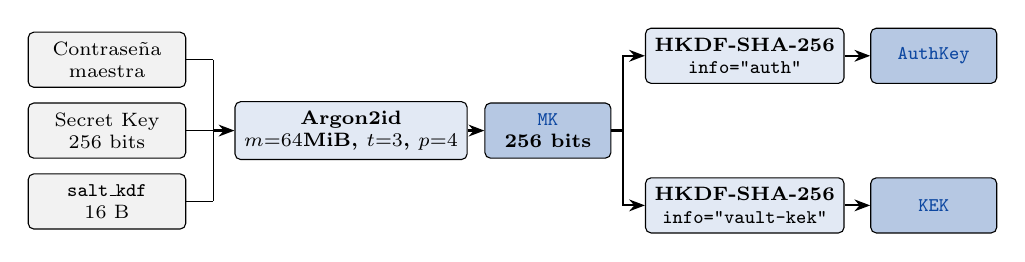
\begin{tikzpicture}[x=1cm, y=1cm]
    \tikzset{dato/.append style={minimum width=20mm},
             op/.append style={minimum width=25mm},
             llave/.append style={minimum width=16mm}}

    \node[dato] (mp)   at (0, 0.9) {Contraseña\\ maestra};
    \node[dato] (sk)   at (0, 0.0) {Secret Key\\ \scriptsize 256 bits};
    \node[dato] (salt) at (0,-0.9) {\texttt{salt\_kdf}\\ \scriptsize 16 B};

    \draw (mp.east)   -- (1.35, 0.9);
    \draw (salt.east) -- (1.35,-0.9);
    \draw (1.35,0.9)  -- (1.35,-0.9);
    \draw (sk.east)   -- (1.35, 0.0);

    \node[op]    (argon) at (3.1, 0.0) {Argon2id\\ \scriptsize $m{=}64$MiB, $t{=}3$, $p{=}4$};
    \node[llave] (mk)    at (5.6, 0.0) {\key{MK}\\ \scriptsize 256 bits};

    \node[op]    (h1) at (8.1, 0.95) {HKDF-SHA-256\\ \scriptsize \texttt{info="auth"}};
    \node[op]    (h2) at (8.1,-0.95) {HKDF-SHA-256\\ \scriptsize \texttt{info="vault-kek"}};
    \node[llave] (ak) at (10.5, 0.95) {\key{AuthKey}};
    \node[llave] (kek) at (10.5,-0.95) {\key{KEK}};

    \draw[flecha] (1.35,0.0) -- (argon.west);
    \draw[flecha] (argon) -- (mk);
    \draw[flecha] (mk.east) -- (6.55, 0.0) -- (6.55, 0.95) -- (h1.west);
    \draw[flecha] (mk.east) -- (6.55, 0.0) -- (6.55,-0.95) -- (h2.west);
    \draw[flecha] (h1) -- (ak);
    \draw[flecha] (h2) -- (kek);
  \end{tikzpicture}

  \vspace{2mm}
  \begin{columns}[T]
    \begin{column}{0.49\textwidth}
      \footnotesize
      \textbf{Detalles de implementación}
      \begin{itemize}
        \item \texttt{salt$'$ = HKDF-Extract(salt\_kdf, SecretKey)}: la Secret Key entra al salt.
        \item Secret Key en formato \texttt{PM1-XXXXX-\ldots} (Base32) con \textbf{checksum de 16 bits}
              que detecta errores al transcribirla.
        \item El cliente \textbf{rechaza parámetros Argon2 débiles} enviados por el servidor
              (dispositivo nuevo: \texttt{GET /kdf-params}).
      \end{itemize}
    \end{column}
    \begin{column}{0.49\textwidth}
      \footnotesize
      \textbf{Lo que se verificó con pruebas}
      \begin{itemize}
        \item Vector de prueba RFC 5869 (HKDF).
        \item \key{AuthKey} $\neq$ \key{KEK}; cambiar contraseña, Secret Key o salt cambia ambas.
        \item Normalización NFKC: la misma contraseña escrita distinto da la misma llave.
        \item Contraseña correcta + Secret Key equivocada $\Rightarrow$ no entra.
      \end{itemize}
    \end{column}
  \end{columns}
\end{frame}

% ---------------------------------------------------------- cifrado de la bóveda
\begin{frame}{Cifrado de la bóveda y \emph{key wrapping}}
  \centering
  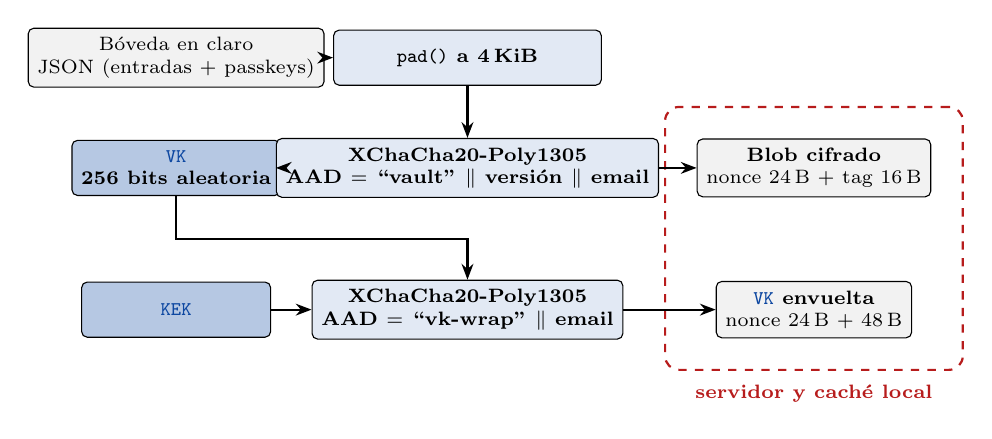
\begin{tikzpicture}[x=1cm, y=1cm]
    \tikzset{dato/.append style={minimum width=24mm},
             op/.append style={minimum width=34mm},
             llave/.append style={minimum width=24mm}}

    \node[dato]  (vault)  at (0.9, 1.6) {Bóveda en claro\\ \scriptsize JSON (entradas + passkeys)};
    \node[op]    (pad)    at (4.6, 1.6) {\texttt{pad()} a 4\,KiB};
    \node[llave] (vk)     at (0.9, 0.2) {\key{VK}\\ \scriptsize 256 bits aleatoria};
    \node[llave] (kek)    at (0.9,-1.6) {\key{KEK}};

    \node[op]   (aead1) at (4.6, 0.2) {XChaCha20-Poly1305\\ \scriptsize AAD $=$ ``vault'' $\Vert$ versión $\Vert$ email};
    \node[dato] (blob)  at (9.0, 0.2) {\textbf{Blob cifrado}\\ \scriptsize nonce 24\,B $+$ tag 16\,B};
    \node[op]   (aead2) at (4.6,-1.6) {XChaCha20-Poly1305\\ \scriptsize AAD $=$ ``vk-wrap'' $\Vert$ email};
    \node[dato] (wvk)   at (9.0,-1.6) {\textbf{\key{VK} envuelta}\\ \scriptsize nonce 24\,B $+$ 48\,B};

    \draw[flecha] (vault) -- (pad);
    \draw[flecha] (pad) -- (aead1);
    \draw[flecha] (vk.east)    -- (aead1.west);
    \draw[flecha] (vk.south)   -- ++(0,-0.55) -| (aead2.north);
    \draw[flecha] (kek.east)   -- (aead2.west);
    \draw[flecha] (aead1) -- (blob);
    \draw[flecha] (aead2) -- (wvk);

    \begin{scope}[on background layer]
      \node[zone, draw=servidor, fit=(blob)(wvk)] (z) {};
    \end{scope}
    \node[font=\scriptsize\bfseries, text=servidor, below=0.5mm of z] {servidor y caché local};
  \end{tikzpicture}

  \vspace{1mm}
  \begin{columns}[T]
    \begin{column}{0.49\textwidth}
      \scriptsize
      \textbf{Qué aporta cada parte del AAD}
      \begin{itemize}
        \item \textbf{versión}: el servidor no puede cambiar el número sin romper el tag.
        \item \textbf{email}: el blob de un usuario no vale como el de otro.
        \item \textbf{etiqueta}: una \key{VK} envuelta nunca se confunde con un blob.
      \end{itemize}
    \end{column}
    \begin{column}{0.49\textwidth}
      \scriptsize
      \textbf{\emph{Padding} (medido)}
      \begin{itemize}
        \item 0, 1 o 10 entradas $\to$ blob de \textbf{4\,112\,B}; 20 $\to$ 8\,208\,B; 40 $\to$ 12\,304\,B.
        \item El relleno va \emph{dentro} del AEAD (autenticado) y los blobs viejos sin relleno
              se siguen abriendo.
      \end{itemize}
    \end{column}
  \end{columns}
\end{frame}

% ---------------------------------------------------------- nonces y AAD en código
\begin{frame}[fragile]{Correctitud: nonces y AAD imposibles de usar mal}
  \begin{columns}[T]
    \begin{column}{0.52\textwidth}
\begin{lstlisting}
# client/crypto/aead.py
def encrypt(key, plaintext, aad):
    """Devuelve (nonce, ciphertext||tag)."""
    nonce = secrets.token_bytes(24)  # siempre fresco
    ct = xchacha20poly1305_encrypt(
        plaintext, aad, nonce, key)
    return nonce, ct

def encode_aad(*fields):
    # prefijo de longitud: ("ab","c") != ("a","bc")
    return b"".join(struct.pack(">I", len(f)) + f
                    for f in fields)
\end{lstlisting}
    \end{column}
    \begin{column}{0.46\textwidth}
      \footnotesize
      \begin{itemize}
        \item \code{encrypt()} \textbf{no acepta un nonce}: lo genera siempre con el CSPRNG.
              La reutilización es imposible desde el código de la aplicación.
        \item Con 192 bits, la colisión de nonces aleatorios es despreciable
              (a diferencia de los 96 bits de AES-GCM).
        \item Todos los AAD y mensajes firmados usan \code{encode\_aad}: sin ambigüedad de
              concatenación.
        \item Salts nuevos en cada registro, cambio de contraseña y exportación.
      \end{itemize}
      \vspace{1mm}
      \begin{block}{\scriptsize Verificado en las pruebas}
        \scriptsize Dos cifrados del mismo texto dan nonces distintos; cambiar \emph{cualquier}
        byte del ciphertext, el AAD, la llave o el nonce hace fallar el descifrado.
      \end{block}
    \end{column}
  \end{columns}
\end{frame}

% ---------------------------------------------------------- passkeys
\begin{frame}{Passkeys Ed25519: protocolo implementado}
  \centering
  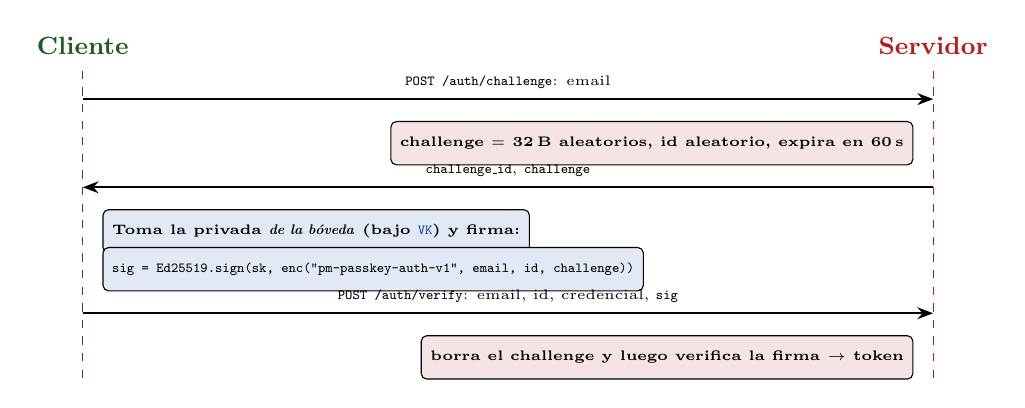
\begin{tikzpicture}[x=1cm, y=0.8cm, font=\scriptsize]
    \tikzset{cbox/.style={op, anchor=west, minimum width=50mm, minimum height=5.5mm, font=\tiny\bfseries},
             sbox/.style={op, fill=servidor!12, anchor=east, minimum width=50mm, minimum height=5.5mm, font=\tiny\bfseries}}
    \node[font=\small\bfseries, text=cliente]  at (0.6, 0) {Cliente};
    \node[font=\small\bfseries, text=servidor] at (11.4,0) {Servidor};
    \draw[dashed, cliente]  (0.6,-0.4) -- (0.6,-5.3);
    \draw[dashed, servidor] (11.4,-0.4) -- (11.4,-5.3);

    \draw[flecha] (0.6,-0.85) -- node[above, font=\tiny] {\texttt{POST /auth/challenge}: email} (11.4,-0.85);
    \node[sbox] at (11.15,-1.55) {challenge $=$ 32\,B aleatorios, id aleatorio, expira en 60\,s};
    \draw[flecha] (11.4,-2.25) -- node[above, font=\tiny] {\texttt{challenge\_id}, \texttt{challenge}} (0.6,-2.25);
    \node[cbox] at (0.85,-2.95) {Toma la privada \emph{de la bóveda} (bajo \key{VK}) y firma:};
    \node[cbox] at (0.85,-3.55) {\texttt{sig = Ed25519.sign(sk, enc("pm-passkey-auth-v1", email, id, challenge))}};
    \draw[flecha] (0.6,-4.25) -- node[above, font=\tiny] {\texttt{POST /auth/verify}: email, id, credencial, \texttt{sig}} (11.4,-4.25);
    \node[sbox] at (11.15,-4.95) {\textbf{borra el challenge} y luego verifica la firma $\to$ token};
  \end{tikzpicture}

  \vspace{1mm}
  \scriptsize
  \begin{columns}[T]
    \begin{column}{0.49\textwidth}
      \textbf{Decisiones de seguridad}
      \begin{itemize}
        \item El challenge se borra \emph{antes} de verificar: un solo uso aunque la firma falle.
        \item Registro con \textbf{prueba de posesión} (firma sobre la llave pública).
        \item Correo inexistente: se responde igual (no enumera usuarios).
        \item \texttt{/auth/verify} comparte el \emph{rate limiting} de \texttt{/login}.
      \end{itemize}
    \end{column}
    \begin{column}{0.49\textwidth}
      \textbf{¿Para qué sirve si la privada está bajo \key{VK}?}
      \begin{itemize}
        \item \textbf{Renovar la sesión} cuando el token (15\,min) expira, sin volver a pedir la contraseña.
        \item \textbf{Desbloquear sin enviar \key{AuthKey}}: la bóveda se abre desde la caché local
              y el servidor sólo recibe una firma.
        \item 30 pruebas: \emph{replay}, challenge expirado, credencial ajena, revocación\ldots
      \end{itemize}
    \end{column}
  \end{columns}
\end{frame}

% ---------------------------------------------------------- anti-rollback
\begin{frame}{Anti-\emph{rollback}: dos capas}
  \begin{columns}[T]
    \begin{column}{0.5\textwidth}
      \small
      \textbf{Capa 1 — versión en el AAD}
      \begin{itemize}\footnotesize
        \item El servidor no puede \emph{relabelar} un blob v2 como v9: el tag Poly1305 falla
              $\Rightarrow$ \texttt{IntegrityError}.
        \item \texttt{PUT /vault} acepta sólo \texttt{versión $=$ actual $+1$}
              (UPDATE atómico); si no, \texttt{409}.
      \end{itemize}
      \vspace{2mm}
      \textbf{Capa 2 — marca de agua en el cliente}
      \begin{itemize}\footnotesize
        \item Cada dispositivo guarda la versión más alta que ya verificó
              (\texttt{max\_version.json}).
        \item Un blob \textbf{íntegro pero viejo} se rechaza con \texttt{RollbackError} en
              \texttt{unlock()} y \texttt{pull()}.
        \item Se compara \emph{después} de validar el tag: el número ya está autenticado.
        \item Si hay rollback no se toca nada: ni caché, ni marca de agua, ni memoria.
      \end{itemize}
    \end{column}
    \begin{column}{0.48\textwidth}
      \scriptsize
      \textbf{Servidor malicioso simulado en las pruebas}
      \vspace{1mm}

      \renewcommand{\arraystretch}{1.1}
      \begin{tabular}{@{}p{0.55\textwidth} p{0.38\textwidth}@{}}
        \toprule
        \textbf{El servidor\ldots} & \textbf{El cliente\ldots} \\
        \midrule
        sirve la v2 cuando ya se vio la v4 & \texttt{RollbackError} \\
        sirve la v2 marcada como v9 & \texttt{IntegrityError} \\
        altera un byte del blob & \texttt{IntegrityError} \\
        sirve la v2 vía passkey & \texttt{RollbackError} \\
        avanza legítimamente a v3 & acepta, marca $\to$ 3 \\
        \bottomrule
      \end{tabular}

      \vspace{2mm}
      \begin{alertblock}{\scriptsize Límites honestos}
        \scriptsize Un dispositivo nuevo confía en la primera versión que ve. Un servidor que
        \emph{retiene} versiones nuevas (congelamiento) no se detecta: es disponibilidad.
      \end{alertblock}
    \end{column}
  \end{columns}
\end{frame}

% ---------------------------------------------------------- cambio de contraseña
\begin{frame}{Cambio de contraseña maestra sin re-cifrar la bóveda}
  \centering
  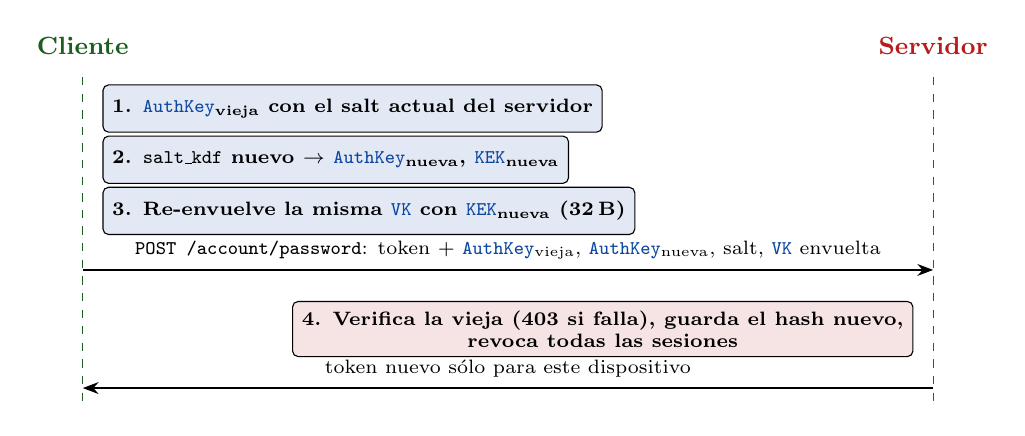
\begin{tikzpicture}[x=1cm, y=1cm, font=\scriptsize]
    \tikzset{cbox/.style={op, anchor=west, minimum width=56mm, minimum height=6mm},
             sbox/.style={op, fill=servidor!12, anchor=east, minimum width=50mm, minimum height=6mm}}
    \node[font=\small\bfseries, text=cliente]  at (0.6, 0) {Cliente};
    \node[font=\small\bfseries, text=servidor] at (11.4,0) {Servidor};
    \draw[dashed, cliente]  (0.6,-0.4) -- (0.6,-4.6);
    \draw[dashed, servidor] (11.4,-0.4) -- (11.4,-4.6);

    \node[cbox] at (0.85,-0.80) {1. \key{AuthKey}$_\text{vieja}$ con el salt actual del servidor};
    \node[cbox] at (0.85,-1.45) {2. \texttt{salt\_kdf} nuevo $\to$ \key{AuthKey}$_\text{nueva}$, \key{KEK}$_\text{nueva}$};
    \node[cbox] at (0.85,-2.10) {3. Re-envuelve \textbf{la misma} \key{VK} con \key{KEK}$_\text{nueva}$ (32\,B)};

    \draw[flecha] (0.6,-2.85) -- node[above, align=center, font=\scriptsize]
      {\texttt{POST /account/password}: token $+$ \key{AuthKey}$_\text{vieja}$, \key{AuthKey}$_\text{nueva}$, salt, \key{VK} envuelta}
      (11.4,-2.85);
    \node[sbox, align=center] at (11.15,-3.60)
      {4. Verifica la vieja (403 si falla), guarda el hash nuevo,\\ \textbf{revoca todas las sesiones}};
    \draw[flecha] (11.4,-4.35) -- node[above, font=\scriptsize] {token nuevo sólo para este dispositivo} (0.6,-4.35);
  \end{tikzpicture}

  \vspace{1mm}
  \begin{columns}[T]
    \begin{column}{0.49\textwidth}
      \scriptsize
      \textbf{Qué NO cambia (verificado en pruebas)}
      \begin{itemize}
        \item El blob: mismo ciphertext, misma versión, misma \key{VK}.
        \item La Secret Key.
      \end{itemize}
      \textbf{Por qué se pide la contraseña vieja además del token:} un token robado no basta
      para apropiarse de la cuenta.
    \end{column}
    \begin{column}{0.49\textwidth}
      \scriptsize
      \textbf{Interacción con passkeys (encontrada al integrar)}
      \begin{itemize}
        \item Tras un cambio hecho en \emph{otro} dispositivo, la contraseña vieja $+$ passkey
              daba una sesión en línea. Se corrigió: tras el login con passkey se exige que la
              contraseña sea la vigente (salt del servidor $+$ \key{VK} recién descargada).
      \end{itemize}
    \end{column}
  \end{columns}
\end{frame}

% ---------------------------------------------------------- tránsito
\begin{frame}{Seguridad en tránsito y \emph{certificate pinning}}
  \begin{columns}[T]
    \begin{column}{0.5\textwidth}
      \small
      \textbf{Canal}
      \begin{itemize}\footnotesize
        \item \textbf{TLS 1.3 mínimo} en cliente y servidor: una conexión TLS 1.2 se rechaza.
        \item Cabeceras: HSTS, \texttt{nosniff}, \texttt{no-store}, CSP; sin cabecera \texttt{Server}.
        \item Tokens de 256 bits, 15\,min, guardados como SHA-256.
        \item \emph{Rate limiting}: 5 fallos por (IP, correo) en 5\,min $\to$ \texttt{429}.
        \item Correo inexistente: verificación contra un hash señuelo y salt falso determinista
              (no se puede enumerar usuarios).
      \end{itemize}
      \vspace{1mm}
      \textbf{Pinning por llave pública (SPKI)}
      \begin{itemize}\footnotesize
        \item \texttt{pin = "sha256//" + Base64(SHA-256(SPKI))}, formato de HPKP / curl.
        \item Se verifica justo tras el handshake, \textbf{antes de enviar un byte HTTP}.
        \item Varios pines: llave actual $+$ respaldo para rotar.
      \end{itemize}
    \end{column}
    \begin{column}{0.48\textwidth}
      \scriptsize
      \textbf{Prueba con servidores TLS reales}
      \vspace{1mm}

      Una CA de prueba firma dos certificados \emph{válidos} para \texttt{127.0.0.1}:
      el legítimo y el de un atacante (CA comprometida).

      \vspace{1mm}
      \renewcommand{\arraystretch}{1.1}
      \begin{tabular}{@{}p{0.52\textwidth} p{0.42\textwidth}@{}}
        \toprule
        \textbf{Escenario} & \textbf{Resultado} \\
        \midrule
        Sin pin, servidor atacante & conecta (MITM) \\
        Con pin, servidor atacante & \texttt{CertificatePinningError}; \textbf{0 peticiones} llegan \\
        Con pin, servidor legítimo & conecta \\
        Pin incorrecto $+$ respaldo correcto & conecta \\
        \bottomrule
      \end{tabular}

      \vspace{2mm}
      \begin{block}{\scriptsize No es ``sin conexión''}
        \scriptsize Un MITM detectado \textbf{no} activa el modo sin conexión: el usuario ve el
        aviso en vez de que la app abra la caché en silencio.
      \end{block}
    \end{column}
  \end{columns}
\end{frame}

% ---------------------------------------------------------- reposo
\begin{frame}{Seguridad en reposo y en el dispositivo}
  \begin{columns}[T]
    \begin{column}{0.5\textwidth}
      \small
      \textbf{Servidor}
      \begin{itemize}\footnotesize
        \item Sólo blob AEAD, \key{VK} envuelta, salts, Argon2id(\key{AuthKey}), llaves públicas
              y SHA-256 de los tokens.
        \item Una prueba busca contraseñas, servicios y la privada de la passkey en la BD:
              \textbf{no aparecen}.
      \end{itemize}
      \textbf{Cliente}
      \begin{itemize}\footnotesize
        \item Caché local cifrada igual que en el servidor (permite abrir sin conexión).
        \item Secret Key en archivo con permisos \texttt{0600}; escrituras atómicas.
        \item Bóveda en claro sólo en RAM mientras está abierta.
      \end{itemize}
    \end{column}
    \begin{column}{0.48\textwidth}
      \small
      \textbf{Uso diario}
      \begin{itemize}\footnotesize
        \item \textbf{Bloqueo automático} por inactividad (5\,min por defecto, de 30\,s a 1\,h;
              no se puede desactivar).
        \item \textbf{Portapapeles}: se borra a los 30\,s (5\,s--5\,min) y al bloquear,
              \emph{sólo} si aún contiene lo que copió la app (se compara su SHA-256).
        \item \textbf{Respaldo \texttt{.pmx}}: Argon2id de una contraseña propia, salt y nonce
              nuevos, encabezado completo en el AAD; las passkeys no se exportan.
      \end{itemize}
    \end{column}
  \end{columns}
\end{frame}

% ---------------------------------------------------------- verificación
\begin{frame}{Verificación: pruebas y análisis estático}
  \begin{columns}[T]
    \begin{column}{0.47\textwidth}
      \centering\scriptsize
      \textbf{144 pruebas automáticas (\texttt{pytest})}
      \vspace{1mm}

      \begin{tabular}{@{}l r@{}}
        \toprule
        \textbf{Archivo} & \textbf{Pruebas} \\
        \midrule
        \texttt{test\_passkeys.py}           & 30 \\
        \texttt{test\_padding\_export.py}    & 23 \\
        \texttt{test\_crypto.py}             & 18 \\
        \texttt{test\_pinning.py} (TLS real) & 13 \\
        \texttt{test\_autolock\_clipboard.py} & 11 \\
        \texttt{test\_server.py}, \texttt{test\_generator.py}, & \\
        \quad\texttt{test\_change\_password.py} & 9 c/u \\
        \texttt{test\_end\_to\_end.py}       & 8 \\
        \texttt{test\_rollback.py}, \texttt{test\_vault.py} & 7 c/u \\
        \bottomrule
      \end{tabular}
    \end{column}
    \begin{column}{0.51\textwidth}
      \small
      \textbf{Análisis estático y dependencias}
      \begin{itemize}\footnotesize
        \item \texttt{bandit -r client server}: \textbf{0 hallazgos}. Tres falsos positivos
              anotados con \texttt{\# nosec} y su justificación (p.\,ej. el prefijo
              \texttt{"PM1"} no es una contraseña).
        \item \texttt{pip-audit}: \textbf{0 vulnerabilidades conocidas} en las dependencias fijadas.
        \item \texttt{semgrep} (reglas \texttt{python}, \texttt{secrets}, \texttt{owasp-top-ten}):
              configurado en GitHub Actions junto con las pruebas, \texttt{bandit} y \texttt{pip-audit}.
      \end{itemize}
      \textbf{Pruebas como ataques}
      \begin{itemize}\footnotesize
        \item Servidor malicioso: blob alterado, viejo o relabelado.
        \item MITM con CA comprometida; \emph{replay} de challenges.
        \item Vector RFC 5869; alteración de cada byte del AEAD.
      \end{itemize}
    \end{column}
  \end{columns}
\end{frame}

% ---------------------------------------------------------- demo
\begin{frame}{Demo: guion}
  \centering\scriptsize
  \renewcommand{\arraystretch}{1.05}
  \begin{tabular}{@{}c p{0.42\textwidth} p{0.46\textwidth}@{}}
    \toprule
    & \textbf{Acción en la app} & \textbf{Qué evidencia criptográficamente} \\
    \midrule
    1 & Crear cuenta y ver el kit de emergencia & Secret Key generada en el cliente; el servidor guarda sólo
        \texttt{\$argon2id\$\ldots} y un blob opaco (consulta a la BD). \\
    2 & Agregar entradas y guardar & La versión sube; el blob sigue en 4\,112\,B (\emph{padding}). \\
    3 & Abrir en un ``dispositivo nuevo'' & Sin Secret Key no entra, aunque la contraseña sea correcta. \\
    4 & Alterar un byte del blob en la BD & El tag Poly1305 falla: \texttt{IntegrityError}. \\
    5 & Devolver un blob viejo desde la BD & \texttt{RollbackError}: la versión ya vista era mayor. \\
    6 & Cambiar el pin (\texttt{PM\_PINS}) & El login muestra el aviso de MITM; no cae al modo sin conexión. \\
    7 & Crear passkey y desbloquear con ella & En el log del servidor aparecen \texttt{/auth/challenge} y
        \texttt{/auth/verify}, pero \textbf{no} \texttt{/login}: \key{AuthKey} no viaja. \\
    8 & Cambiar la contraseña maestra & El ciphertext del blob no cambia; sólo la \key{VK} envuelta. \\
    9 & Copiar una contraseña y esperar & El portapapeles se borra; la bóveda se bloquea por inactividad. \\
    \bottomrule
  \end{tabular}
\end{frame}

% ---------------------------------------------------------- amenazas
\begin{frame}{Análisis de amenazas: diseño $\to$ implementación $\to$ evidencia}
  \centering\scriptsize
  \renewcommand{\arraystretch}{0.95}
  \begin{tabular}{@{}p{0.27\textwidth} p{0.37\textwidth} p{0.29\textwidth}@{}}
    \toprule
    \textbf{Amenaza} & \textbf{Mitigación implementada} & \textbf{Evidencia} \\
    \midrule
    Filtración de la BD & Zero-knowledge; Argon2id(\key{AuthKey}); tokens hasheados & búsqueda de secretos en la BD \\
    Manipulación del blob & Poly1305 sobre blob y \key{VK} envuelta & alteración de cada byte \\
    \emph{Rollback} / \emph{replay} & versión en AAD $+$ marca de agua $+$ 409 & \texttt{test\_rollback.py} \\
    MITM con CA comprometida & TLS 1.3 $+$ pin SPKI & \texttt{test\_pinning.py} (TLS real) \\
    Fuerza bruta \emph{offline} & Argon2id 64\,MiB $+$ Secret Key de 256 bits & parámetros mínimos forzados \\
    Adivinación en línea & \emph{rate limiting} en login, passkeys y cambio de contraseña & prueba de \texttt{429} \\
    Servidor baja los parámetros KDF & el cliente rechaza parámetros débiles & \texttt{WeakKdfParamsError} \\
    Enumeración de usuarios & salt falso determinista, hash señuelo, challenge igual & respuestas idénticas \\
    Reutilización de nonce & \code{encrypt()} sin parámetro de nonce & nonces distintos \\
    Token robado & 15\,min; cambio de contraseña exige la actual y revoca sesiones & \texttt{test\_change\_password.py} \\
    Exposición en el equipo & bloqueo automático, portapapeles temporizado & \texttt{test\_autolock\_clipboard.py} \\
    \bottomrule
  \end{tabular}
\end{frame}

% ---------------------------------------------------------- desviaciones
\begin{frame}{Desviaciones respecto al diseño (y por qué)}
  \centering\scriptsize
  \renewcommand{\arraystretch}{1.05}
  \begin{tabular}{@{}p{0.27\textwidth} p{0.27\textwidth} p{0.38\textwidth}@{}}
    \toprule
    \textbf{Diseño (Entrega 1)} & \textbf{Implementado} & \textbf{Motivo} \\
    \midrule
    UI en PySide6 & Flet 1.1 & UI más moderna; las operaciones lentas corren en hilos y no congelan la ventana. \\
    Python 3.12 & Python 3.10 (CI en 3.12) & versión disponible en el entorno de desarrollo. \\
    PostgreSQL & SQLite por defecto & sin instalación para la demo; PostgreSQL con sólo cambiar \texttt{PM\_DATABASE\_URL}. \\
    Docker Compose & pendiente & se priorizó la criptografía y sus pruebas. \\
    Bloqueo progresivo en \texttt{/login} & ventana deslizante (5 fallos / 5 min) & más simple, mismo objetivo. \\
    Secret Key en el llavero del SO & archivo con permisos \texttt{0600} & portabilidad entre sistemas. \\
    Kit de emergencia en PDF & copiar $+$ confirmación obligatoria & alcance de la UI. \\
    Pinning de ``huella'' & pin de la \textbf{llave pública} (SPKI) & sobrevive a la renovación del certificado. \\
    \bottomrule
  \end{tabular}
\end{frame}

% ---------------------------------------------------------- limitaciones
\begin{frame}{Limitaciones y trabajo futuro}
  \begin{columns}[T]
    \begin{column}{0.52\textwidth}
      \footnotesize
      \textbf{Limitaciones}
      \begin{itemize}
        \item \textbf{Cliente comprometido} sigue siendo juego terminado.
        \item \textbf{Memoria}: Python no permite borrar con garantía \texttt{bytes}/\texttt{str}
              inmutables; al bloquear sólo se sueltan las referencias.
        \item \textbf{Flet} dibuja la UI en un proceso Flutter aparte: lo que se ve en pantalla
              pasa por un canal local entre procesos.
        \item \textbf{Anti-rollback}: confianza en el primer uso y congelamiento no detectable.
        \item \textbf{Cambio de contraseña}: la \key{VK} no rota; un dispositivo sin conexión
              sigue abriendo su caché con la contraseña vieja.
        \item \textbf{Padding}: oculta el número de entradas dentro de bloques de 4\,KiB, no
              la frecuencia de sincronización.
        \item \textbf{Portapapeles}: el historial del SO (Win\,+\,V) puede guardar una copia.
      \end{itemize}
    \end{column}
    \begin{column}{0.46\textwidth}
      \footnotesize
      \textbf{Trabajo futuro}
      \begin{itemize}
        \item Docker Compose con PostgreSQL.
        \item Rotación de \key{VK} (re-cifrar la bóveda) como opción ante compromiso.
        \item Resolución de conflictos por entrada en vez de ``recargar y repetir''.
        \item Revocar passkeys de otros dispositivos al cambiar la contraseña.
        \item Guardar la Secret Key en el llavero del SO.
        \item Kit de emergencia imprimible y TOTP como segundo factor.
      \end{itemize}
    \end{column}
  \end{columns}
\end{frame}

% ---------------------------------------------------------- reparto
\begin{frame}{Reparto del trabajo}
  \begin{columns}[T]
    \begin{column}{0.49\textwidth}
      \begin{block}{\small Franco Pacheco}
        \footnotesize
        \begin{itemize}
          \item Motor criptográfico (Argon2id, HKDF, AEAD, \emph{key wrapping}) y Secret Key.
          \item Servidor: registro, login, blob versionado, TLS 1.3.
          \item Passkeys Ed25519 (cliente y servidor).
          \item Anti-\emph{rollback} en el cliente.
          \item \emph{Certificate pinning} por SPKI.
          \item Interfaz en Flet.
        \end{itemize}
      \end{block}
    \end{column}
    \begin{column}{0.49\textwidth}
      \begin{block}{\small Andy Rai Berru Tenorio}
        \footnotesize
        \begin{itemize}
          \item Cambio de contraseña maestra (cliente y \texttt{/account/password}).
          \item Bloqueo automático por inactividad.
          \item Limpieza segura del portapapeles.
          \item \emph{Padding} del blob.
          \item Exportación e importación cifrada \texttt{.pmx}.
          \item Preferencias de seguridad y diálogos de cuenta.
        \end{itemize}
      \end{block}
    \end{column}
  \end{columns}
  \vspace{2mm}
  \centering
  {\footnotesize Integración por \emph{pull requests}; la revisión cruzada encontró y corrigió la
  interacción entre passkeys y cambio de contraseña.}
\end{frame}

% ---------------------------------------------------------- cierre
\begin{frame}{Resumen}
  \begin{itemize}
    \item Implementamos el gestor \textbf{zero-knowledge} diseñado: el servidor almacena, pero
          nunca entiende.
    \item Todo lo prometido como P0 y P1 está hecho; de P2 falta sólo Docker Compose.
    \item La criptografía se apoya en librerías auditadas y en una API que hace difícil usarla
          mal (nonces internos, AAD con prefijo de longitud, mensajes con etiqueta de dominio).
    \item Cada defensa tiene una prueba que la ataca: servidor malicioso, MITM con CA
          comprometida, \emph{replay}, alteración de bytes.
    \item Las limitaciones están documentadas, incluidas las que encontramos al integrar.
  \end{itemize}
  \vspace{4mm}
  \centering
  {\Large ¿Preguntas?}
\end{frame}

\end{document}
